\chapter{Kinetic Theory: Boltzmann, Kac and Propagation of Chaos}
\label{ch:kinetic}

\section{From Maxwell to Lanford}

Maxwell's paper of 1860~\cite{maxwell1860} derived the velocity distribution of a gas from symmetry and independence and computed the viscosity, finding to his own surprise that it is independent of density. His 1867 paper~\cite{maxwell1867} introduced the transfer equations for moments and the special inverse fifth power force law, the Maxwell molecules, for which the moment equations close. Boltzmann's paper of 1872~\cite{boltzmann1872} wrote down the equation for the one particle density, proved the $H$ theorem, and claimed thereby to have derived the second law of thermodynamics from mechanics. Loschmidt objected in 1876~\cite{loschmidt1876} that the mechanical equations are time reversible, so for every motion that increases entropy the reversed motion decreases it. Zermelo objected in 1896~\cite{zermelo1896}, using Poincar\'e's theorem, that the mechanical motion is recurrent. Boltzmann's replies, developed in the 1877 counting paper~\cite{boltzmann1877} and in the \emph{Vorlesungen \"uber Gastheorie}~\cite{boltzmann1896}, moved the argument from individual trajectories to probabilities: the $H$ theorem is a statement about typical behavior, and the hypothesis of molecular chaos is a statement about the measure on initial conditions.

Hilbert in 1912~\cite{hilbert1912} brought the integral equation methods to the linearized collision operator. Carleman in 1933~\cite{carleman1933} proved the first existence theorem for the spatially homogeneous equation. Grad introduced the moment method in 1949~\cite{grad1949} and identified the low density scaling, now called the Boltzmann Grad limit, in 1958~\cite{grad1958}. Kac in 1956~\cite{kac1956} replaced the mechanics by a stochastic model in which molecular chaos could be proved. Lanford in 1975~\cite{lanford1975} proved the derivation for hard spheres over a short time. DiPerna and Lions in 1989~\cite{diperna1989} proved global existence of renormalized solutions. Deng, Hani and Ma in 2024 extended Lanford's theorem to long times~\cite{denghanima2024}.

\section{The Boltzmann equation}

For a density $f(t,x,v)\geq0$ on $\R^d_x\times\R^d_v$ the Boltzmann equation is
\begin{gather*}
\partial_tf+v\cdot\nabla_xf = \alpha\,Q(f,f), \\
Q(f,f)(v) = \int_{\R^d}\int_{S^{d-1}}B(v-v_*,\sigma)\big(f'f'_*-ff_*\big)\dd\sigma\dd v_*,
\end{gather*}
where $f = f(v)$, $f_* = f(v_*)$, $f' = f(v')$, $f'_* = f(v'_*)$, and the post collisional velocities are
\[
v' = \frac{v+v_*}{2}+\frac{|v-v_*|}{2}\sigma,\qquad v'_* = \frac{v+v_*}{2}-\frac{|v-v_*|}{2}\sigma.
\]
The collision rate $\alpha>0$, which equals $N\varepsilon^{d-1}$ in the Boltzmann Grad scaling below, sets the time scale and is taken equal to one in the spatially homogeneous statements of this section. The collision kernel $B\geq0$ depends only on $|v-v_*|$ and the angle $\theta$ between $v-v_*$ and $\sigma$. The hard sphere collision operator of Chapter~\ref{ch:hilbert}, which is written there with the unit vector $\omega$ of \eqref{eq:hs_collision} and the weight $((v-v_*)\cdot\omega)_+$, is the operator $Q$ above with $B = 2^{1-d}|v-v_*|(\sin\frac\theta2)^{3-d}$, which is $B = \frac14|v-v_*|$ for $d = 3$: the substitution $\sigma = (v-v_*-2((v-v_*)\cdot\omega)\omega)/|v-v_*|$ turns $((v-v_*)\cdot\omega)_+\dd\omega$ into $B\dd\sigma$ and $v-((v-v_*)\cdot\omega)\omega$ into $v'$. The change of variables $(v,v_*,\sigma)\mapsto(v',v'_*,\sigma')$ with $\sigma' = (v-v_*)/|v-v_*|$ has unit Jacobian and preserves $B$, and the swap $(v,v_*,\sigma)\mapsto(v_*,v,-\sigma)$ is likewise measure preserving, preserves $B$ and exchanges $v'$ with $v'_*$.

\begin{lemma}[Weak form]
\label{lem:weakform}
For any test function $\varphi(v)$ for which the integrals converge,
\[
\int Q(f,f)\varphi\dd v = \frac12\iiint B\,ff_*\big(\varphi'+\varphi'_*-\varphi-\varphi_*\big)\dd\sigma\dd v_*\dd v.
\]
\end{lemma}

\begin{proof}
Write $\int Q\varphi = \iiint B(f'f'_*-ff_*)\varphi$. The swap $(v,v_*,\sigma)\mapsto(v_*,v,-\sigma)$ leaves $B$, $ff_*$ and $f'f'_*$ unchanged and exchanges $\varphi$ with $\varphi_*$; averaging yields $\frac12\iiint B(f'f'_*-ff_*)(\varphi+\varphi_*)$. The pre and post collisional change of variables maps $f'f'_*-ff_*$ to its negative and $\varphi+\varphi_*$ to $\varphi'+\varphi'_*$; averaging the last integral with its image gives $\frac14\iiint B(f'f'_*-ff_*)(\varphi+\varphi_*-\varphi'-\varphi'_*)$. The same change of variables turns $\iiint Bf'f'_*(\varphi+\varphi_*-\varphi'-\varphi'_*)$ into $\iiint Bff_*(\varphi'+\varphi'_*-\varphi-\varphi_*)$, so the two terms of this integral are equal, and their sum is the claim.
\end{proof}

Taking $\varphi\in\{1,v_1,\dots,v_d,|v|^2\}$, for which $\varphi'+\varphi'_* = \varphi+\varphi_*$ by conservation of momentum and energy, shows that mass, momentum and energy are conserved. These are the collision invariants.

\begin{lemma}[Collision invariants]
\label{lem:collision_invariants}
If $\varphi$ is measurable and $\varphi(v')+\varphi(v'_*) = \varphi(v)+\varphi(v_*)$ for almost every $(v,v_*,\sigma)$, then $\varphi(v) = a+b\cdot v+c|v|^2$ for constants $a\in\R$, $b\in\R^d$, $c\in\R$.
\end{lemma}

\begin{proof}[Proof for continuous $\varphi$]
The pairs $(v',v'_*)$ obtained from $(v,v_*)$ as $\sigma$ ranges over the sphere are exactly the pairs with the same sum and the same sum of squares, so the hypothesis says that $\varphi(v)+\varphi(w) = \varphi(v')+\varphi(w')$ whenever $v+w = v'+w'$ and $|v|^2+|w|^2 = |v'|^2+|w'|^2$. Subtracting the constant $\varphi(0)$ we may assume $\varphi(0) = 0$.

Step one: if $v\perp w$, the pair $(v+w,0)$ has the same sum and sum of squares as $(v,w)$, so $\varphi(v+w) = \varphi(v)+\varphi(w)$. Thus $\varphi$ is additive on orthogonal vectors.

Step two: the even part $g(v) = \frac12(\varphi(v)+\varphi(-v))$ is radial, since $(v,-v)$ and $(u,-u)$ have the same sum and sum of squares whenever $|u| = |v|$. Write $g(v) = G(|v|^2)$. Additivity on orthogonal vectors gives $G(a+b) = G(a)+G(b)$ for all $a,b\geq0$, and a continuous additive function on $[0,\infty)$ is linear: $G(s) = cs$.

Step three: the odd part $k(v) = \frac12(\varphi(v)-\varphi(-v))$ is continuous, odd and, as in step two, additive on orthogonal vectors. Let $v$ and $w$ be nonzero vectors pointing in the same direction, and choose $u\perp v$ with $|u|^2 = v\cdot w$, which is possible because $d\geq2$. Then $v+u\perp w-u$, because $(v+u)\cdot(w-u) = v\cdot w-|u|^2 = 0$, while $u\perp v$ and $-u\perp w$, so additivity on orthogonal vectors and oddness give $k(v+w) = k(v+u)+k(w-u) = k(v)+k(u)+k(w)+k(-u) = k(v)+k(w)$. If $w = -\tau v$ with $\tau>0$, apply this to the pair $((1-\tau)v,\tau v)$ when $\tau<1$ and to the pair $(v,(\tau-1)v)$ when $\tau>1$, and use oddness; for $\tau = 1$ the claim is $k(0) = 0$. Hence $k$ is additive on each line through the origin, and since it is continuous, $k(sv) = sk(v)$ for real $s$. For arbitrary $v$ and $w$ write $w = w_\parallel+w_\perp$ with $w_\parallel$ parallel to $v$ and $w_\perp\perp v$. Then $w_\perp$ is orthogonal to $v+w_\parallel$ and to $w_\parallel$, so $k(v+w) = k(v+w_\parallel)+k(w_\perp) = k(v)+k(w_\parallel)+k(w_\perp) = k(v)+k(w)$. Thus $k$ is additive and homogeneous, hence linear: $k(v) = b\cdot v$ with $b_i = k(e_i)$.

Combining, $\varphi(v) = \varphi(0)+b\cdot v+c|v|^2$. For measurable $\varphi$ one first mollifies in the velocity variables, which preserves the functional equation, and then passes to the limit.
\end{proof}

\section{The \texorpdfstring{$H$}{H} theorem}

\begin{theorem}[Boltzmann]
\label{thm:htheorem}
Let $f$ be a smooth, positive, rapidly decaying solution of the spatially homogeneous equation $\partial_tf = Q(f,f)$, and let $H(f) = \int f\log f\dd v$. Then
\begin{gather*}
\frac{\dd}{\dd t}H(f) = -D(f), \\
D(f) = \frac14\iiint B\,\big(f'f'_*-ff_*\big)\log\frac{f'f'_*}{ff_*}\dd\sigma\dd v_*\dd v\geq0,
\end{gather*}
and $D(f) = 0$ if and only if $f$ is a Maxwellian, $f(v) = \rho(2\pi\theta)^{-d/2}\exp(-|v-u|^2/2\theta)$.
\end{theorem}

\begin{proof}
$\frac{\dd}{\dd t}H = \int Q(f,f)(1+\log f)$, and Lemma~\ref{lem:weakform} with $\varphi = \log f$ gives $\frac12\iiint Bff_*\log\frac{f'f'_*}{ff_*}$, while the term from $\varphi = 1$ vanishes. Applying the pre and post collisional change of variables once more and averaging produces $-D(f)$. The integrand of $D$ has the form $(x-y)(\log x-\log y)\geq0$, so $D\geq0$, with equality only if $f'f'_* = ff_*$ almost everywhere, that is, $\log f$ is a collision invariant. Lemma~\ref{lem:collision_invariants} gives $\log f = a+b\cdot v+c|v|^2$, and integrability forces $c<0$.
\end{proof}

Boltzmann's $H$ is the negative of the entropy $S(f) = -\int f\log f\dd v$ of Chapter~\ref{ch:entropy}. The $H$ theorem is therefore the second law for the Boltzmann equation: the entropy $S$ increases along solutions. Its quantitative version, the rate at which $H(f)-H(M)$ decays, was the subject of Cercignani's conjecture that $D(f)\geq\lambda\,(H(f)-H(M))$; Bobylev and Cercignani~\cite{bobylevcercignani1999} showed that it fails in general, and Villani~\cite{villani2003cercignani} proved the weaker bound $D(f)\geq C_\varepsilon(H(f)-H(M))^{1+\varepsilon}$ for a wide class of kernels. Desvillettes and Villani~\cite{desvillettesvillani2005} proved convergence to equilibrium for the inhomogeneous equation at almost exponential rates, provided the solution remains smooth.

\section{Hard spheres and the BBGKY hierarchy}

The rigorous derivation starts from the Liouville equation for $N$ hard spheres of diameter $\varepsilon$. Let $F_N(t,z_1,\dots,z_N)$, $z_i = (x_i,v_i)$, be the symmetric density on the phase space with exclusion $|x_i-x_j|>\varepsilon$, transported by the hard sphere flow with the reflection rule \eqref{eq:hs_collision}. The $s$ particle marginals $F^{(s)}_N$ satisfy the Bogoliubov, Born, Green, Kirkwood and Yvon hierarchy
\[
\partial_tF^{(s)}_N+\sum_{i\leq s}v_i\cdot\nabla_{x_i}F^{(s)}_N = (N-s)\varepsilon^{d-1}\,C_{s,s+1}F^{(s+1)}_N,
\]
where the collision operator $C_{s,s+1}$ integrates $F^{(s+1)}$ over the sphere of contact between one of the first $s$ particles and particle $s+1$, weighted by the relative velocity, with gain and loss terms distinguished by whether the configuration is pre or post collisional. In the Boltzmann Grad scaling $N\varepsilon^{d-1} = \alpha$ the prefactor tends to $\alpha$, the excluded volume vanishes, and the hierarchy formally becomes the Boltzmann hierarchy
\[
\partial_tf^{(s)}+\sum_{i\leq s}v_i\cdot\nabla_{x_i}f^{(s)} = \alpha\,C^0_{s,s+1}f^{(s+1)},
\]
which has the factorized solution $f^{(s)} = f^{\otimes s}$ precisely when $f$ solves the Boltzmann equation. Propagation of chaos at this level is uniqueness for the Boltzmann hierarchy plus convergence of the BBGKY solutions to it.

\begin{theorem}[Lanford]
\label{thm:lanford}
Let $f_0$ be a probability density on $\R^d\times\R^d$ with $f_0(x,v)\leq Ce^{-\beta|v|^2/2}$ and continuous. Let $F_{N,0}$ be the restriction of $f_0^{\otimes N}$ to the hard sphere phase space, normalized. There is $T^*>0$, depending only on $C$, $\beta$ and $\alpha$, such that for every $s$ the marginals $F^{(s)}_N(t)$ converge as $N\to\infty$, $N\varepsilon^{d-1} = \alpha$, locally uniformly outside a null set, to $f(t)^{\otimes s}$, where $f$ is the solution of the Boltzmann equation with the hard sphere kernel and initial datum $f_0$, for all $t\in[0,T^*]$.
\end{theorem}

The time $T^*$ is a fraction of the mean free time. The proof, which we only sketch, writes the solution of each hierarchy as a Duhamel series. Writing $S_s(t)$ for the free flow of $s$ hard spheres, iteration of the integrated hierarchy gives
\[
\begin{multlined}F^{(s)}_N(t) = \sum_{k=0}^{N-s}\alpha_N^k\int_0^t\!\!\int_0^{t_1}\!\!\cdots\!\!\int_0^{t_{k-1}}S_s(t-t_1)C_{s,s+1}S_{s+1}(t_1-t_2)\cdots\\ \cdots C_{s+k-1,s+k}S_{s+k}(t_k)F^{(s+k)}_{N,0}\,\dd t_k\cdots\dd t_1,\end{multlined}
\]
with $\alpha_N = (N-s)\varepsilon^{d-1}$, and the Boltzmann hierarchy has the same expansion with free flows and collision operators of point particles. Each term is an integral over collision trees with $k$ branchings. In weighted norms the $k$th term is bounded by $(Ct)^k$ times a constant, because the collision operators lose a factor $|v|$ that the Gaussian weight controls at the cost of a geometric factor; the series therefore converges for $t<T^* = 1/C$. The proof then compares the two series term by term over collision trees, bounds the series uniformly in $N$ by a Cauchy Kovalevskaya argument in weighted spaces, which forces $T^*$ small, and then shows that the series converge term by term, the key geometric estimate being that recollisions, in which two particles that have already interacted meet again, occupy a vanishing fraction of phase space. Gallagher, Saint Raymond and Texier~\cite{gst2013} gave a complete modern proof with quantitative rates, and extended it to short range potentials. We prove only the abstract Cauchy Kovalevskaya lemma, Lemma~\ref{lem:cauchy_kovalevskaya}, and outline the rest; the original proof is in Lanford~\cite{lanford1975}, and a complete proof is also in Cercignani, Illner and Pulvirenti~\cite{cip1994}.

Lanford's theorem gives a rigorous version of Boltzmann's reply to Loschmidt's paradox for data that are chaotic at time zero. The irreversibility appears in the limit, because the set of configurations that would reverse is a null set in the limit measure: chaos is propagated forward in time but not backward, since post collisional velocities are correlated. Order matters: the theorem fixes $t$ and lets $N\to\infty$; for fixed $N$ Poincar\'e recurrence still holds.

The restriction to short times was removed by Deng, Hani and Ma~\cite{denghanima2024}.

\begin{theorem}[Deng, Hani and Ma]
\label{thm:dhm}
Let $d\geq2$, let $\beta>0$, and let $f_0$ be a probability density such that $f_0$ and $\nabla_xf_0$ have finite norm $\sum_{k\in\Z^d}\sup_{|x-k|\leq1,\,v\in\R^d}e^{2\beta|v|^2}|g(x,v)|$, where $g$ stands for $f_0$ or $\nabla_xf_0$. Suppose that the solution $f$ of the Boltzmann equation with the hard sphere kernel, $\alpha = 1$ and initial datum $f_0$ exists on $[0,T]$ and satisfies $\sup_{x,v}e^{2\beta|v|^2}f(t,x,v)\leq A$ for all $t\in[0,T]$. Draw the initial state of the hard sphere gas from the grand canonical ensemble with density $f_0$ and $\varepsilon^{-(d-1)}$ particles on average: the number $N$ of particles is random and, given $N$, the initial state has density proportional to $\prod_{j\leq N}f_0(z_j)$ on the non overlapping configurations. There is $\kappa>0$, depending only on $d$, such that for $\varepsilon$ small enough, depending on $d$, $\beta$, $T$, $A$ and the norm of $f_0$, for all $t\in[0,T]$ and all $s\leq|\log\varepsilon|$, the rescaled $s$ particle correlation function $f_s(t)$ of the gas is within $\varepsilon^\kappa$ in $L^1$ of $f(t)^{\otimes s}$ restricted to the non overlapping configurations.
\end{theorem}

We quote this theorem without proof, as Theorem~1 of Deng, Hani and Ma~\cite{denghanima2024}, and describe the ideas of its proof below; the torus version and the fluid limits are in the companion paper~\cite{denghanima2025}, treated in Chapter~\ref{ch:hydro}. Theorem~\ref{thm:dhm} differs from Theorem~\ref{thm:lanford} in the ensemble, the mode of convergence and the time. If the solution is global and bounded, the proof allows $T$ to grow with $\varepsilon$ like $\log|\log\varepsilon|$.

The difficulty in going beyond Lanford's time is that the bound on the Duhamel series is only geometric. The number of collision trees with $k$ branchings grows like $k!$, the time ordered integrals contribute $t^k/k!$, and the product is the bound $(Ct)^k$ above. Beyond $T^*$ the bound gives no control, and the same holds for the Duhamel expansion of the Boltzmann equation itself. Deng, Hani and Ma subdivide $[0,T]$ into time layers, short enough for the Boltzmann solution to be given on each layer by a convergent series, and propagate from layer to layer a cumulant ansatz that records the correlations created by the earlier collisions. The cumulants are shown to be small in $L^1$ by a combinatorial analysis of the collision histories, drawn as diagrams that they call molecules, and by a cutting algorithm. The strategy adapts to particles the long time derivation of the wave kinetic equation by Deng and Hani~\cite{denghani2023}.

\section{Lanford windows}

The time $T^*$ of Theorem~\ref{thm:lanford} is the precise boundary of what the classical proof achieves and the reason a long time theory was needed. We call $[0,T^*]$ a Lanford window. Its existence and size follow from an abstract Cauchy Kovalevskaya argument in a scale of Banach spaces.

\begin{lemma}[Abstract Cauchy Kovalevskaya]
\label{lem:cauchy_kovalevskaya}
Let $(X_r)_{0<r\leq r_0}$ be Banach spaces with $X_r\subset X_{r'}$ and $\|\cdot\|_{r'}\leq\|\cdot\|_r$ for $r'<r$. For each $t\geq0$ let $A(t)$ be a linear operator that maps $X_r$ into $X_{r'}$ for $r'<r\leq r_0$, with $t\mapsto A(t)u$ continuous into $X_{r'}$ for $u\in X_r$, and such that, for all $t\geq0$ and all $r'<r\leq r_0$,
\[
\|A(t)u\|_{r'}\leq\frac{K}{r-r'}\,\|u\|_r.
\]
Then for $u_0\in X_{r_0}$ and $0<r<r_0$ the series
\[
u(t) = \sum_{k\geq0}\int_{0<t_k<\dots<t_1<t}A(t_1)\cdots A(t_k)u_0\dd t_k\cdots\dd t_1
\]
converges in $X_r$ for $0\leq t<T_r = \frac{r_0-r}{eK}$, and it solves $u' = A(t)u$ with $u(0) = u_0$ there, with values in $X_{r'}$ for every $r'<r$.
\end{lemma}

\begin{proof}
Fix $k\geq1$ and split $[r,r_0]$ into $k$ equal intervals of length $\delta/k$, $\delta = r_0-r$. Applying the hypothesis $k$ times, each time losing $\delta/k$,
\[
\|A(t_1)\cdots A(t_k)u_0\|_r\leq\Big(\frac{Kk}{\delta}\Big)^k\|u_0\|_{r_0}\qquad\text{for all }t_1,\dots,t_k.
\]
The simplex $0<t_k<\dots<t_1<t$ has volume $t^k/k!$, and $k^k\leq e^kk!$, so the $k$th term $u_k(t)$ of the series satisfies $\|u_k(t)\|_r\leq\big(\frac{eKt}{\delta}\big)^k\|u_0\|_{r_0}$, a geometric series that converges for $t<\delta/(eK)$. Since $u_k(t) = \int_0^tA(s)u_{k-1}(s)\dd s$ and $\|A(s)u_{k-1}(s)\|_{r'}\leq\frac{K}{r-r'}\|u_{k-1}(s)\|_r$ for $r'<r$, the series $\sum_kA(s)u_{k-1}(s)$ converges in $X_{r'}$ locally uniformly in $s<T_r$. Hence $u(t) = u_0+\int_0^tA(s)u(s)\dd s$ in $X_{r'}$, which is the equation.
\end{proof}

Lanford applies the lemma to the BBGKY and Boltzmann hierarchies with the scale of norms
\[
\|F\|_{\beta,\gamma} = \sup_{s\geq1}\sup_{Z_s}e^{\gamma s}\,e^{\beta E(Z_s)}\,|F^{(s)}(Z_s)|,\qquad E(Z_s) = \frac12\sum_{i\leq s}|v_i|^2,
\]
which measure Gaussian decay in velocity and exponential decay in the number of particles. The generator of each hierarchy contains the free transport, which is unbounded in these norms, and one passes to the interaction picture. The free flow $S(t)$ preserves $E(Z_s)$ and is therefore an isometry of $\|\cdot\|_{\beta,\gamma}$, so $u(t) = S(-t)F(t)$ solves $u' = A(t)u$ with $A(t) = S(-t)\,C\,S(t)$, where $C$ collects the collision operators $C_{s,s+1}$, and the series of the lemma is the Duhamel series of the hierarchy. The collision operator $C_{s,s+1}$ integrates over the velocity of the added particle and multiplies by a relative velocity, so it costs one factor $\beta^{-d/2}$ from the Gaussian integral, one factor of $s$ from the sum over particles, and one factor $\sum_{i\leq s}|v_i|+|v_{s+1}|$ from the cross section. The factors of $s$ and of velocity are absorbed by giving up a little decay: since $s\,e^{-\eta s}\leq(e\eta)^{-1}$ and $\sum_i|v_i|\,e^{-\eta E}\leq C\sqrt{s/\eta}$, decreasing $\gamma$ and $\beta$ by amounts proportional to $r-r'$ along a fixed line in the $(\beta,\gamma)$ plane produces exactly the hypothesis of the lemma, with $K$ proportional to $\alpha\beta^{-d/2}$ times a function of $(\beta,\gamma)$. The lemma then gives a window
\[
T^* = \frac{r_0-r}{eK}\;\asymp\;c_d\,\tau_{\mathrm{mf}},
\]
a fixed fraction of the mean free time $\tau_{\mathrm{mf}}\asymp(\alpha\langle|v|\rangle)^{-1}$, independent of $N$. Figure~\ref{fig:lanford} is a schematic of the mechanism.

\begin{figure}[t]
\centering
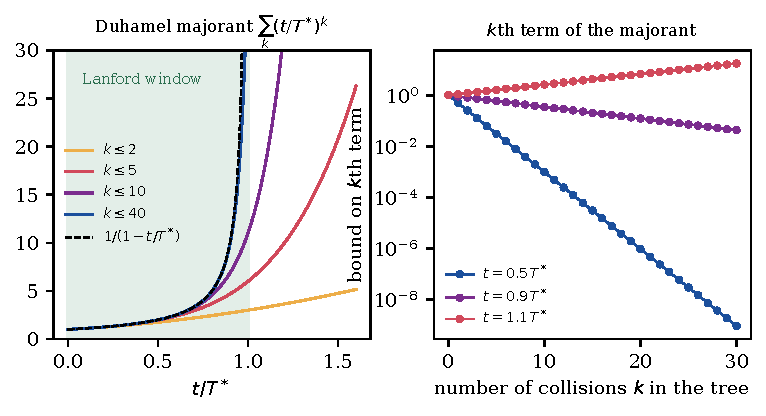
\includegraphics[width=\textwidth]{lanford_window}
\caption{Schematic of the Lanford window. Left, partial sums of the majorant $\sum_k(t/T^*)^k$ of the Duhamel series converge for $t<T^*$ (shaded) to the limit $1/(1-t/T^*)$, drawn dashed, and diverge beyond. Right, the $k$th term $(t/T^*)^k$ of the majorant, a bound on the contribution of collision trees with $k$ branchings, for $t = 0.5\,T^*$, $0.9\,T^*$ and $1.1\,T^*$: it decays geometrically inside the window and grows outside. No hard sphere quantity is computed.}
\label{fig:lanford}
\end{figure}

\subsection{Why windows cannot simply be iterated}

If chaos at time zero implies chaos at time $T^*$, why not restart the argument at $T^*$ and cover any interval by finitely many windows? The obstruction is that the conclusion of the theorem is weaker than its hypothesis. At time zero the $N$ particle law is a product measure restricted to the hard sphere phase space, with bounds in the norm $\|\cdot\|_{\beta,\gamma}$. At time $T^*$ the limit is again a product, but at finite $N$ the law carries correlations created by collisions, of size $O(\varepsilon)$ in a weak sense but not small in the norms the lemma requires, and the decay parameters have been spent: the window was obtained by trading $(\beta_0,\gamma_0)$ for $(\beta,\gamma)$, and the next window would start from worse parameters. A naive iteration therefore produces a sequence of windows whose lengths sum to a finite total.

Three ways around the obstruction are known. At equilibrium the Gibbs measure is invariant, so the a priori bounds at time $T^*$ are as good as at time zero, and many windows can be concatenated. Bodineau, Gallagher, Saint Raymond and Simonella use this invariance, for a gas in a periodic box in dimension at least three, first to show that the covariance of the fluctuations of the empirical measure is governed by the linearized Boltzmann equation globally in time, by a duality method combined with a pruning of the collision trees that removes those with superexponential growth~\cite{bgss2023cpam}, and then to show that the whole fluctuation field converges, for all times, to the solution of the fluctuating Boltzmann equation, by a study of clusters of pseudo trajectories, with quantitative bounds on time intervals that grow, slowly, with the number of particles~\cite{bgss2024}. Away from equilibrium the same authors control fluctuations and large deviations of the empirical measure, but only for short times~\cite{bgss2023}. Near equilibrium, a refinement of Lanford's argument based on estimates of the pathological collision trees gives the Brownian motion of a tagged particle of Chapter~\ref{ch:brownian}, in a diffusive limit~\cite{bgs2016}. Far from equilibrium, Deng, Hani and Ma do iterate short windows, which they call time layers, but they propagate across the layers a cumulant ansatz that records the correlations created in the earlier layers~\cite{denghanima2024}, as described after Theorem~\ref{thm:dhm}.

\subsection{Moment conditioning inside the window}

The initial data of Theorem~\ref{thm:lanford} are products restricted to non overlapping configurations, not data conditioned on moments, and what follows is a heuristic and not a theorem. A gas prepared with prescribed local density, velocity and temperature is, in the language of Chapter~\ref{ch:types}, a large system conditioned on local moments, and the conditional limit theorem suggests that its $k$ particle marginals are close to products of local Maxwellians. Lanford's theorem propagates a product structure for the length of a window, and the $H$ theorem (Theorem~\ref{thm:htheorem}) describes how the one particle law then relaxes toward the Maxwellian determined by the conserved moments. On this reading the passage from atoms to continua has three steps: conditioning on moments produces chaos, Lanford windows propagate chaos, and the Hilbert expansion of Chapter~\ref{ch:hydro} reads off the evolution of the conditioned moments as the equations of fluid dynamics. The three step picture is our framing of the subject: the first step is the heuristic above, and the second and third are Theorems~\ref{thm:lanford} and~\ref{thm:dhm} and the hydrodynamic limits of Chapter~\ref{ch:hydro}.


\section{Kac's model}

Kac~\cite{kac1956} proposed to separate the probabilistic content of Boltzmann's argument from the mechanical one by studying a Markov process whose collisions are random. Consider $N$ particles with one dimensional velocities $v = (v_1,\dots,v_N)$ on the sphere $S^{N-1}(\sqrt N) = \{\sum v_i^2 = N\}$. At rate $N$, a pair $(i,j)$ is chosen uniformly and an angle $\theta$ uniformly on $[0,2\pi)$, and the pair is rotated:
\[
(v_i,v_j)\mapsto(v_i\cos\theta-v_j\sin\theta,\;v_i\sin\theta+v_j\cos\theta).
\]
Energy is conserved, momentum is not. The uniform measure on the sphere is invariant and, by the Maxwell, Poincar\'e and Borel lemma (Theorem~\ref{thm:sphere_lemma}), its one particle marginal converges to the standard Gaussian. The generator acts on symmetric functions, and the master equation for the law $F_N(t)$ is linear.

\begin{theorem}[Kac]
\label{thm:kac}
If $F_N(0)$ is $f_0$ chaotic in the sense of Chapter~\ref{ch:axioms}, then $F_N(t)$ is $f_t$ chaotic for every $t>0$, where $f_t$ solves the Kac Boltzmann equation
\[
\partial_tf(v) = \frac{1}{\pi}\int_{\R}\int_0^{2\pi}\big(f(v')f(w')-f(v)f(w)\big)\dd\theta\dd w,
\]
with $(v',w')$ the rotation of $(v,w)$ by $\theta$.
\end{theorem}

Kac proved the theorem~\cite{kac1956} by expanding the evolution in a power series in time, where the combinatorics of the Markov generator replace the geometry of collisions; the stochasticity removes recollisions as an issue. We quote the theorem without proof. Figure~\ref{fig:kac} shows a simulation started from a bimodal law: the one particle histogram relaxes to the Gaussian and the kurtosis, which is about $1.04$ for the initial law, approaches three. The decay is consistent with the linear recursion for the fourth moment: a single collision maps $m_4$ to $\frac34m_4+\frac34$ when $m_2 = 1$, whose fixed point is the Gaussian value three.

\begin{figure}[t]
\centering
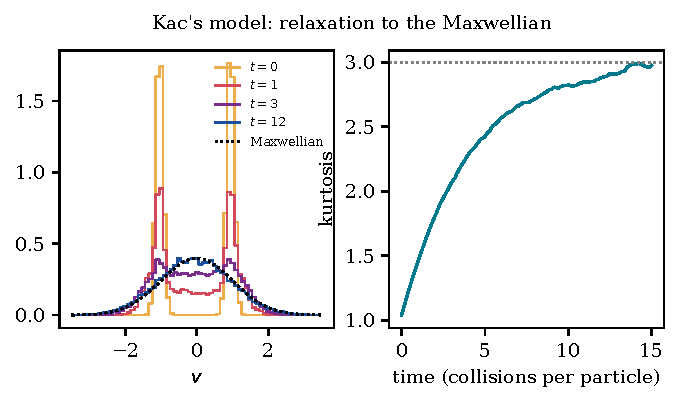
\includegraphics[width=\textwidth]{kac_model}
\caption{Kac's model with $N=20{,}000$ particles. The initial law is an equal mixture of two Gaussian peaks at $\pm1$ with standard deviation $0.1$, scaled to unit second moment. Left, one particle histograms at times $0$, $1$, $3$ and $12$, measured in collisions per particle, with the Maxwellian dotted; right, kurtosis against the same time, with the Gaussian value three dotted.}
\label{fig:kac}
\end{figure}

Kac also proposed a program: prove convergence to equilibrium for the $N$ particle process uniformly in $N$, and deduce convergence for the Boltzmann equation. The spectral gap of the generator is bounded below uniformly in $N$, as shown by Janvresse~\cite{janvresse2001} and computed exactly by Carlen, Carvalho and Loss~\cite{ccl2003}, so the $L^2$ part of the program works. But $L^2$ is the wrong norm, since chaotic densities have $L^2$ norms exponential in $N$; the right quantity is relative entropy, which is extensive, and the entropy production of the $N$ particle process does not control entropy uniformly in $N$. The largest constant $\Gamma_N$ such that the entropy production is at least $\Gamma_N$ times the relative entropy with respect to the uniform law on the sphere, for every initial law of finite relative entropy, is at least $2/(N-1)$ by an argument of Villani~\cite{villani2003cercignani} and tends to zero as $N\to\infty$~\cite{cclv2010}. Gao, Wang and Xia~\cite{gaowangxia2026} prove in a recent preprint that $\Gamma_N = 2/(N-1)$ for every $N\geq2$, which confirms Villani's conjecture that $\Gamma_N$ is of order $1/N$; Open Problem~\ref{prob:kinetic} of Chapter~\ref{ch:open} asks for classes of initial laws on which a constant independent of $N$ exists. Mischler and Mouhot~\cite{mischlermouhot2013} completed a quantitative version of Kac's program, proving propagation of chaos with explicit rates in Wasserstein distance uniformly in time.

\section{Propagation of chaos for mean field diffusions}

A clean case in which propagation of chaos can be proved in a few lines is the mean field diffusion. Let $b:\R^d\times\R^d\to\R^d$ be Lipschitz with constant $L$, in the sense that $|b(x,y)-b(x',y')|\leq L(|x-x'|+|y-y'|)$, and consider
\[
\dd X^i_t = \frac1N\sum_{j=1}^Nb(X^i_t,X^j_t)\dd t+\dd W^i_t,\qquad i = 1,\dots,N,
\]
with independent Brownian motions and independent initial conditions of law $f_0$. The candidate limit is the McKean Vlasov process
\[
\dd\bar X^i_t = \int b(\bar X^i_t,y)\,f_t(\dd y)\dd t+\dd W^i_t,\qquad f_t = \mathrm{Law}(\bar X^i_t),
\]
driven by the same Brownian motion and started at the same point. For Lipschitz $b$ and $\E|X^i_0|^2<\infty$ the McKean Vlasov equation has a unique solution~\cite{sznitman1991}, and the $\bar X^i$ are independent and identically distributed. The coupling argument below is due to Sznitman~\cite{sznitman1991}. It is a different result from Theorem~\ref{thm:sznitman}, from the same lectures, which relates chaos to the convergence of empirical measures.

\begin{theorem}[McKean Vlasov coupling]
\label{thm:mckean}
Assume that $\E|X^i_0|^2<\infty$. For every $T$ there is $C_T$, depending only on $L$, $T$, $d$ and $\E|X^i_0-\E X^i_0|^2$, such that
\[
\sup_{t\leq T}\E|X^i_t-\bar X^i_t|\leq\frac{C_T}{\sqrt N}.
\]
Consequently the $k$ particle marginals of $(X^1_t,\dots,X^N_t)$ converge to $f_t^{\otimes k}$ in the Wasserstein distance $W_1$ for the metric $\sum_{i\leq k}|x_i-y_i|$, uniformly in $t\leq T$ and at rate $kC_T/\sqrt N$.
\end{theorem}

\begin{proof}
Subtracting the equations,
\[
|X^i_t-\bar X^i_t|\leq\int_0^t\Big|\frac1N\sum_jb(X^i_s,X^j_s)-\int b(\bar X^i_s,y)f_s(\dd y)\Big|\dd s.
\]
Insert $\frac1N\sum_jb(\bar X^i_s,\bar X^j_s)$. The Lipschitz bound controls the first difference by $\frac{L}{N}\sum_j(|X^i_s-\bar X^i_s|+|X^j_s-\bar X^j_s|)$, whose expectation is $2L\,\E|X^1_s-\bar X^1_s|$ by exchangeability. The second difference is an average of $N$ terms $b(\bar X^i_s,\bar X^j_s)-\int b(\bar X^i_s,y)f_s(\dd y)$. Put $V_T = \sup_{s\leq T}\E|\bar X^1_s-\E\bar X^1_s|^2$. For $j\neq i$ the terms are, conditionally on $\bar X^i_s$, centered and independent, with conditional variance at most $L^2V_T$; the term $j = i$ is at most $L\int|\bar X^i_s-y|f_s(\dd y)$ in absolute value, which has mean at most $L\sqrt{2V_T}$. By the Cauchy Schwarz inequality the mean absolute value of the second difference is at most $(1+\sqrt2)L\sqrt{V_T/N}\leq3L\sqrt{V_T/N}$. Hence $\psi(t) = \E|X^1_t-\bar X^1_t|$ satisfies $\psi(t)\leq\int_0^t\big(2L\psi(s)+3L\sqrt{V_T/N}\big)\dd s$, and Gr\"onwall's lemma gives $\psi(t)\leq\frac32\sqrt{V_T/N}\,(e^{2Lt}-1)$.

It remains to bound $V_T$, and this is where the second moment of $f_0$ enters. Let $\bar X$ and $\bar X'$ be independent copies of the McKean Vlasov process, with Brownian motions $W$ and $W'$, and $D = \bar X-\bar X'$. The drift $x\mapsto\int b(x,y)f_s(\dd y)$ is $L$ Lipschitz, so $|D_s|\leq|D_0|+\sup_{r\leq s}|W_r-W'_r|+L\int_0^s|D_r|\dd r$. Gr\"onwall's lemma and Doob's inequality give $\E|D_s|^2\leq2e^{2Ls}(2v_0+8ds)$ with $v_0 = \E|X^i_0-\E X^i_0|^2$, and $\E|\bar X_s-\E\bar X_s|^2 = \frac12\E|D_s|^2$, so $V_T\leq e^{2LT}(2v_0+8dT)$. Replacing $V_T$ by this bound in the estimate of $\psi$ gives the theorem with $C_T = \frac32\sqrt{e^{2LT}(2v_0+8dT)}\,(e^{2LT}-1)$, which depends only on $L$, $T$, $d$ and $v_0$.
\end{proof}

The coupling proof is the simplest instance of a principle that runs through this book. A many particle system is compared with $N$ independent copies of a nonlinear one particle process; the comparison is a law of large numbers for the empirical measure, and the error is the fluctuation, of order $N^{-1/2}$. The same structure governs particle filters, ensemble Kalman filters and the particle approximations of generative flows in Part~\ref{part:statmech}.

\section{The arrow of time: Kac's ring}

Kac devised an exactly solvable model in which both Boltzmann's prediction and its failure can be seen~\cite{kac1959}. Place $N$ sites on a circle, each holding a ball that is white or black. A fixed subset of $m$ edges between adjacent sites is marked. At each time step every ball moves one site clockwise, and a ball crossing a marked edge changes color. Let $N^w_t$ and $N^b_t$ be the numbers of white and black balls. Boltzmann's reasoning, which assumes that the color of the ball about to cross an edge is independent of whether the edge is marked, the analogue of the \emph{Stosszahlansatz}, predicts with $\mu = m/N$
\begin{gather*}
N^w_{t+1}-N^b_{t+1} = (1-2\mu)(N^w_t-N^b_t), \\
\frac{N^w_t-N^b_t}{N} = (1-2\mu)^t\,\frac{N^w_0-N^b_0}{N},
\end{gather*}
exponential relaxation to equal numbers of each color. But the dynamics is deterministic and reversible, and after $2N$ steps every ball has crossed every edge twice, so the configuration returns exactly: the recurrence time is $2N$, and after $N$ steps every ball has crossed all $m$ marked edges once, so if $m$ is odd the colors are exactly reversed.

Figure~\ref{fig:kacring} shows the model: for $t$ much smaller than $N$ the trajectory follows Boltzmann's prediction closely. Kac showed that if the marked set is chosen at random, Boltzmann's prediction holds for most marked sets, for each fixed $t$, as $N\to\infty$: the fluctuations of $(N^w_t-N^b_t)/N$ about $(1-2\mu)^t$ are of order $N^{-1/2}$. The arrow of time is a law of large numbers over the disorder, valid for times small compared with the recurrence time. This is precisely the structure of Lanford's theorem, and the content of Boltzmann's reply to Zermelo.

\begin{figure}[t]
\centering
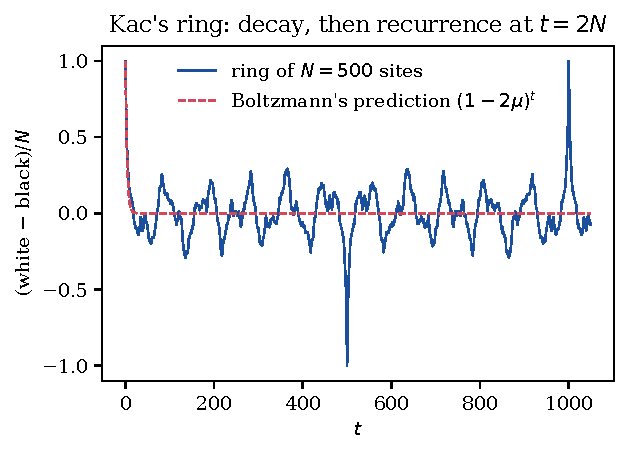
\includegraphics[width=0.92\textwidth]{kac_ring}
\caption{Kac's ring with $N=500$ sites and $61$ marked edges, started with all balls white. The deterministic dynamics follows Boltzmann's exponential law, then reverses at $t=N$ and recurs at $t=2N$.}
\label{fig:kacring}
\end{figure}

\section{Ergodic theorems}

The other classical route to justifying averages is ergodic theory. Its basic results, Birkhoff's pointwise ergodic theorem (Theorem~\ref{thm:birkhoff}) and von Neumann's mean ergodic theorem (Theorem~\ref{thm:vonneumann}), are proved in Chapter~\ref{ch:ergodic}.

Sinai proved in 1970~\cite{sinai1970} that dispersing billiards are ergodic, and Sim\'anyi proved the Boltzmann Sinai ergodic hypothesis for hard ball systems on tori in stages: for typical hard disk systems in 2003~\cite{simanyi2003}, for typical hard ball systems in 2004~\cite{simanyi2004}, in general under a technical assumption in 2009~\cite{simanyi2009}, and without that assumption in 2013~\cite{simanyi2013}. Ergodicity, however, is the wrong tool for the sixth problem. It speaks about time averages of a single system over times comparable to recurrence times, while the kinetic limit concerns ensemble averages over times of order the mean free time, for typical initial conditions, as the number of particles diverges. Lanford's theorem uses no ergodic theory. In the language of Chapter~\ref{ch:axioms}, it is a statement about the de Finetti measure of the gas, and its probabilistic content is that independence, once assumed, propagates.

\section{The Lorentz gas: a derivation valid for all times}

There is one kinetic limit in which the restriction to short times disappears. In the Lorentz gas a single particle moves among fixed spherical scatterers of radius $\varepsilon$ placed at the points of a Poisson process of intensity $\varepsilon^{-(d-1)}$, reflecting elastically. Gallavotti showed in 1969~\cite{gallavotti1969}, and Spohn~\cite{spohn1978} and Boldrighini, Bunimovich and Sinai~\cite{bbs1983} extended the result, that in the Boltzmann Grad limit the law of the particle, averaged over the scatterers, converges for all times to the solution of the linear Boltzmann equation
\[
\partial_tf+v\cdot\nabla_xf = \int_{S^{d-1}}\big(f(v')-f(v)\big)\,|v|\,b(\omega)\dd\omega.
\]
The linear equation describes a particle whose velocity jumps at the times of a Poisson process, a Markov process in phase space. The difficulty of Lanford's theorem, recollisions between moving particles, is replaced by the possibility of returning to a scatterer already visited, and since the scatterers are Poisson distributed and the particle explores new territory, such returns have vanishing probability on every bounded time interval. The theorem shows that the Markov property, the essence of Boltzmann's assumption, emerges from deterministic dynamics in a random medium. Averaging over the medium is a de Finetti average, and the Poisson law of the scatterers is the prior that makes the limit Markov.

For a periodic arrangement of scatterers the result fails: Golse~\cite{golse2008} showed that the limit is not described by the linear Boltzmann equation, and Marklof and Str\"ombergsson~\cite{marklof2011} identified the correct limit, a generalized kinetic equation with memory, using ergodic theory on homogeneous spaces. The randomness of the medium matters, which is another form of Poincar\'e's observation that the irreversible limit is a statement about a probability measure on initial conditions.

\section{Mean field limits and the Vlasov equation}

When the interaction is long range and weak rather than short range and strong, the kinetic limit is the Vlasov equation
\[
\partial_tf+v\cdot\nabla_xf-(\nabla W*\rho_f)\cdot\nabla_vf = 0,\qquad\rho_f = \int f\dd v,
\]
for particles interacting through a potential $W$ scaled by $1/N$. Braun and Hepp in 1977~\cite{braunhepp1977} and Dobrushin in 1979~\cite{dobrushin1979} proved the mean field limit for smooth $W$ by a stability estimate in Wasserstein distance: two solutions of the Vlasov equation, and in particular an empirical measure of the $N$ particle system and the true solution, separate at most exponentially in time in $W_1$. Dobrushin's estimate is the deterministic counterpart of the coupling argument of Theorem~\ref{thm:mckean}. The singular case of the Coulomb interaction, relevant to plasmas and galaxies, was long out of reach; the modulated energy method of Serfaty~\cite{serfaty2020} gives mean field limits for Coulomb and Riesz interactions, for gradient and conservative first order flows and, for Newton's law, in the monokinetic case. The Vlasov equation is reversible, and its long time behavior, Landau damping, is a mixing phenomenon in velocity space proved in the nonlinear setting by Mouhot and Villani~\cite{mouhotvillani2011}. It is a second route to irreversibility, through phase mixing rather than collisions.

\section{Grad's moment method and the closure problem}

Integrating the Boltzmann equation against polynomials in $v$ yields an infinite hierarchy of moment equations, each involving the next. Grad's thirteen moment method of 1949~\cite{grad1949} closes the hierarchy by assuming that $f$ is a local Maxwellian times a polynomial of degree three determined by thirteen moments: density, velocity, temperature, stress and heat flux. The resulting hyperbolic system reproduces Navier Stokes Fourier in the hydrodynamic limit and extends it into the transition regime, but it can lose hyperbolicity and produce unphysical shocks. Levermore's maximum entropy closures~\cite{levermore1996} replace the polynomial ansatz by the density maximizing entropy subject to the moment constraints, an exponential family, which guarantees hyperbolicity and an entropy inequality at the cost of nonpolynomial fluxes. Closure problems in kinetic theory, in turbulence modeling and in approximate Bayesian inference, where variational families play the role of the closure ansatz, are versions of the same question: which low dimensional family best represents a high dimensional law consistent with known averages.

\section*{Exercises}
\begin{enumerate}
\item Verify that the pre and post collisional change of variables in Lemma~\ref{lem:weakform} has unit Jacobian.
\item For Kac's model, derive the differential equation satisfied by the fourth moment under the normalization of Theorem~\ref{thm:kac}, and solve it.
\item In Kac's ring with $N$ sites and $m$ marked edges, show that the configuration at time $N$ is the color reversal of the initial one when $m$ is odd and equal to it when $m$ is even.
\item In dimension one, take $b(x,y) = Ly$ and $f_0 = N(0,s^2)$ in Theorem~\ref{thm:mckean}. Compute $\E|X^i_t-\bar X^i_t|$ exactly and show that it is at least $\sqrt{2/\pi}\,(e^{Lt}-1)s/\sqrt N$, so that $C_T$ must depend on the variance of $f_0$.
\item Show that the linear Boltzmann equation conserves mass and kinetic energy but not momentum, and identify its equilibria.
\end{enumerate}


\section*{Notes}

Cercignani, Illner and Pulvirenti~\cite{cip1994} is the classical text on the mathematical theory of dilute gases. Villani's review~\cite{villani2002review} is the standard survey of the mathematics of the Boltzmann equation. Gallagher's article in the Bulletin~\cite{gallagher2019} explains the passage from Newton to Navier Stokes, and the Bourbaki expos\'e of Bodineau, Gallagher, Saint Raymond and Simonella~\cite{bgss2026} explains the proof of Deng, Hani and Ma.
